\documentclass[fleqn]{article}
\usepackage{mathtools}
\usepackage{graphicx}
\usepackage{amssymb}
\usepackage[margin = 0.75in]{geometry}
\usepackage{enumerate}
\usepackage{color}
\usepackage{fancyvrb}
\usepackage{breqn}
\usepackage{fancyhdr}
\usepackage{multicol}
%\usepackage[latin1]{inputenc}
\usepackage{tikz}

\renewcommand{\thispagestyle}[1]{}
\pagestyle{fancy}
\lhead{\textbf{NAME:}}
\rhead{}

\begin{document}
\title{Math 120R.002 Exam 2 Version B}
\date{10.23.15}
\author{Instructor: Ammon Washburn}
\maketitle

\section*{Instructions:} 
Please show all of your work for each question. Providing just the final answer \textbf{will not merit full credit}. The best way to ensure full credit is to provide the equation you use, show some work, and mark your final answer in an obvious way (circle, box, underline, etc.). The point values for each question are located at the beginning of the question.

\vspace{1in} 

\begin{tabular}{|p{6.5in}|} 
\hline 
\noindent By signing my name below, I agree that I am following all rules and regulations set forth by the Code of Academic Integrity.  Furthermore, I agree that I am following all rules set by my instructor and by the course policy for this exam.  This includes ensuring that all calculator programs except possibly QUADRATIC FORMULA have been deleted.\\
\vspace{.3 in}\\
\underline{Signature:	\hspace{2.5 in}	Date:\hspace{1.25 in}}\\
\hline 
\end{tabular} 

\pagebreak
\thispagestyle{fancy}{
\lhead{}
\rhead{/22}}



\section*{Free Response}

\begin{enumerate}
\item \textit{(9 points)} Consider the following graph.
Assume all the functions are of the form $y = a\cdot b^x$. \\
\vspace{0.25in}
\begin{minipage}{0.55\textwidth}
\begin{enumerate}
\item Which function has the smallest $b$ value?

\vspace{0.7in}

\item Which functions have the same $a$ value?

\vspace{0.7in}

\item Which function(s) have $b > 1$?

\vspace{0.7in}

\item As $x \to \infty$, $h(x) \to $ \underline{\hspace{1in}}.
\end{enumerate}
\end{minipage}
\begin{minipage}{0.4\textwidth}
\begin{tikzpicture}[y=0.2cm, x=1cm]
	\draw[<->] (-3.2,0) -- (3.2,0) node[right] {$x$};
	\draw[<->] (0,-6) -- (0,31) node[above] {$y$};
	\draw[thick,smooth,samples=100,domain=-3.0:1.3,color=black,<->] plot (\x, 5*4^\x);
	\draw[thick,smooth,samples=100,domain=-2.6:3.0,color=black,dotted,<->] plot (\x, 5*0.5^\x);
	\draw[thick,smooth,samples=100,domain=-3.0:3.0,color=black,dashed,<->] plot (\x, 2*2^\x);
	\node [left] at (-1, 10) {$h(x)$};
	\node [right] at (1, 20) {$f(x)$};
	\node [right] at (2, 8) {$g(x)$};
\end{tikzpicture}
\end{minipage}

\vspace{0.5in}

\item \textit{(9 points)} Consider the following logarithmic function $g(x) = -\log_{2}(3x-2)$
\begin{enumerate}
\item What is the domain and range of $g(x)$?

\vspace{1.5in}

\item What is the vertical asymptote of $g(x)$?

\vspace{1in}

\end{enumerate}

\pagebreak
\thispagestyle{fancy}{
\lhead{}
\rhead{/15}}

\item \textit{(15 points)} Consider the polynomial $P(x) = -x^5 + 6x^4 - 10x^3 + 4x^2$.
\begin{enumerate}
\item
The leading term is \underline{\hspace{1in}}, which indicates that as $x \to +\infty$, $y \to $ \underline{\hspace{1in}}, and as $x \to -\infty$, $y \to $ \underline{\hspace{1in}}.

\item Given that $c = 2$ is a zero of $P(x)$, write $P(x)$ in factored form with \textbf{exact} values for all roots. 

\vspace{3.25in}

\item State the $y-$intercept of $P(x)$ as a coordinate.

\vspace{0.5in}

\item Use the axes provided to draw an \textbf{accurate} sketch of $P(x)$.

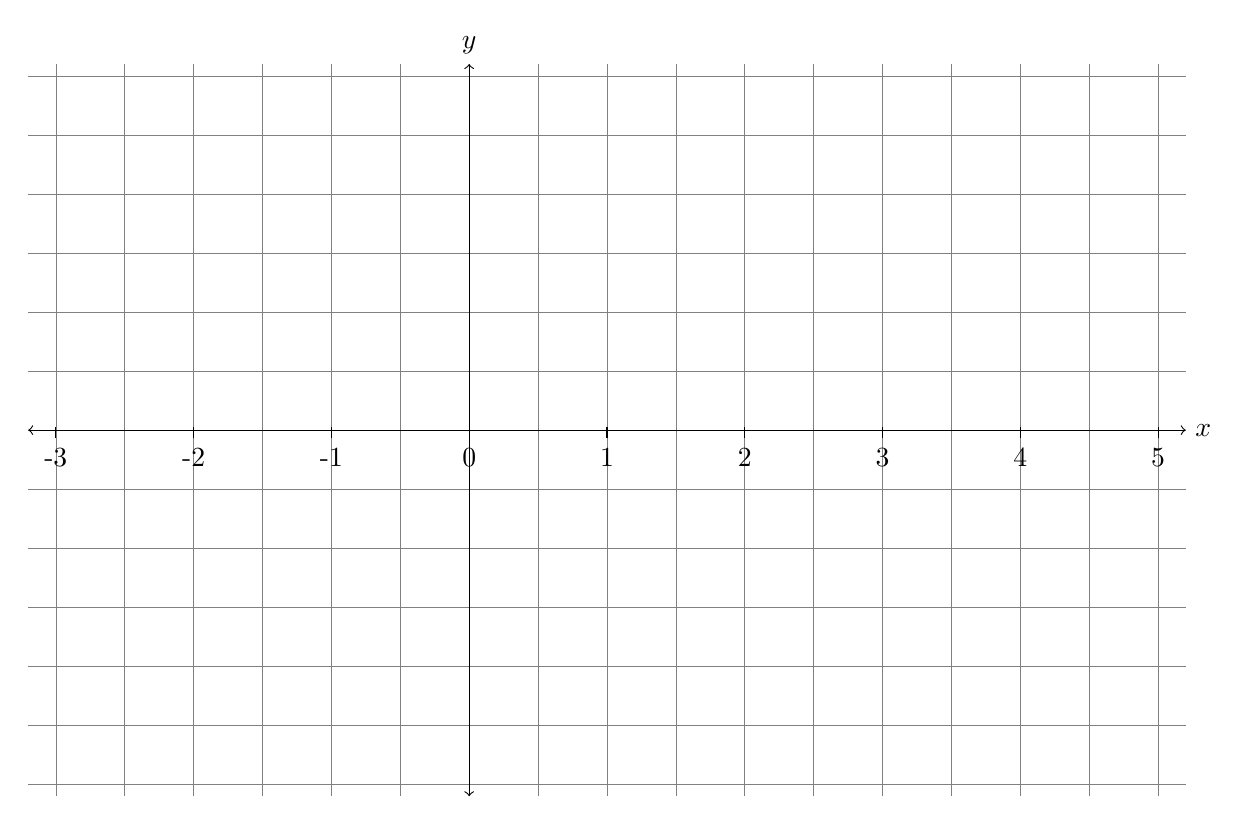
\begin{tikzpicture}[y=0.15cm, x=1.75cm]
	\draw[very thin,color=gray, xstep=0.5, ystep=5] (-3.2,-31) grid (5.2,31);
	\draw[<->] (-3.2,0) -- (5.2,0) node[right] {$x$};
	\draw[<->] (0,-31) -- (0,31) node[above] {$y$};
\foreach \x in {-3, ..., 5}
	\draw (\x, 1pt) -- (\x, -3pt) node[anchor=north] {\x};
\end{tikzpicture}

\end{enumerate}

\pagebreak
\thispagestyle{fancy}{
\lhead{}
\rhead{/15}}

\item 
\textit{(15 points)} Consider the rational function 
\begin{align*}
r(x) &= \frac{ 4x^2+8x-12 }{ 5x^2+5x-10 }
\end{align*}
Find the following quantities, if they exist. 
If they do not, write NONE.
\begin{enumerate}
\item $x-$intercept(s)

\vspace{1.25in}

\item $y-$intercept(s)

\vspace{1.25in}

\item Vertical asymptote(s)

\vspace{1.25in}

\item Hole(s)

\vspace{1.25in}

\item Horizontal and/or Slant asymptote(s)

\end{enumerate}

\pagebreak
\thispagestyle{fancy}{
\lhead{}
\rhead{/18}}

\item 
\textit{(12 points)} A man with an ice cream shop wants to change the price of his ice cream sandwiches so that he makes more revenue.  With the sandwiches currently priced at \$5 he sells on average 750 sandwiches.  After some careful experiments, he predicts for every dollar increase the sandwiches sales decrease by 50.
\begin{enumerate}
\item What is the equation that models revenue $R(x)$ as a function of the \textit{increase} in sandwich price $x$

\vspace{1in}

\item What is the price that gives the maximum revenue?  What is the maximum revenue?

\vspace{2in}
Price:  \underline{\hspace{2in}} \qquad Max revenue: \underline{\hspace{2in}}

\end{enumerate}

\vspace{0.5in}

\item \textit{(10 points)} Suppose you want to invest money in an account with an interest rate of 5\% per year.
How many years will it take for your initial investment to double if the interest is compounded continuously?

\vspace{1.25in}

\pagebreak
\thispagestyle{fancy}{
\lhead{}
\rhead{/30}
\rfoot{/100}}

\section*{Multiple Choice}

\item \textit{(6 points)} Determine the exponential function $f(x) = Cb^x$ that passes through the points $(0,4)$ and $(2,1)$
\begin{enumerate}
\item $f(x) = 4(2)^x$
\item $f(x) = 2(4)^x$
\item $f(x) = 4(-2)^x$
\item $f(x) = 4(\frac{1}{2})^x$
\item $f(x) = 8(\frac{1}{2})^x$
\end{enumerate}

\vspace{0.5in}

\item \textit{(6 points)} Find the value of $c$ such that $(x + 1)$ is a factor of $h(x) = x^5-c x^4+x^3+105 x^2-74 x-168$.
\begin{multicols}{3}
\begin{enumerate}
\item -75
\item 75
\item 9
\item 0
\item None of these answers
\end{enumerate}
\end{multicols}

\vspace{0.5in}

\item \textit{(6 points)} let $H(t) = -x^2+4x+21$.  What is the maximum value for $H$?
\begin{multicols}{3}
\begin{enumerate}
\item Max value: 2
\item Max value: 7
\item Max value: 21
\item Max value: 25
\item Max value: 30
\item There is no maximum value
\end{enumerate}
\end{multicols}

\vspace{0.5in}

\item \textit{(6 points)} Determine $A$ so that the following function has a horizontal asymptote at $y=3$: $f(x) = \frac{10x^2+2}{Ax^2 -3}$
\begin{multicols}{3}
\begin{enumerate}
\item $A = \frac{2}{3}$
\item $A = \frac{3}{10}$
\item $A = -\frac{3}{2}$
\item $A = \frac{10}{3}$
\item $A = 0$
\end{enumerate}
\end{multicols}

\vspace{.5in}

\item \textit{(6 points)} Suppose $P(x) = -x^3(x^2+89)(-x-13)^3$. Determine which one of the following options
correctly describes the end behavior of the graph $y = P(x)$.
\begin{enumerate}
\item $y \rightarrow +\infty$ as $x \rightarrow -\infty$ and $y \rightarrow +\infty$ as $x \rightarrow +\infty$
\item $y \rightarrow -\infty$ as $x \rightarrow -\infty$ and $y \rightarrow +\infty$ as $x \rightarrow +\infty$
\item $y \rightarrow +\infty$ as $x \rightarrow -\infty$ and $y \rightarrow -\infty$ as $x \rightarrow +\infty$
\item $y \rightarrow -\infty$ as $x \rightarrow -\infty$ and $y \rightarrow -\infty$ as $x \rightarrow +\infty$
\end{enumerate}


\end{enumerate}

\end{document}